Risk-based adalah suatu metode yang digunakan untuk mengukur dan mengelola risiko. Dalam konteks keamanan, risk-based authentication adalah metode autentikasi yang mengukur tingkat risiko dari suatu permintaan akses, dan mengambil tindakan yang sesuai berdasarkan tingkat risiko tersebut. Metode ini bertujuan untuk mengenali dan menangani ancaman potensial tanpa mengekang fleksibilitas dan kenyamanan pengguna (Smith \& Jones, 2020). 

Dalam konteks Machine-to-Machine (M2M) authentication, risk-based authentication digunakan untuk mengukur tingkat risiko dari suatu permintaan akses dan mengambil tindakan yang sesuai berdasarkan tingkat risiko tersebut (Chen et al., 2018). Prosesnya dapat dilakukan dengan cara menganalisis faktor-faktor yang dapat meningkatkan risiko, seperti lokasi geografis, waktu akses, dan jenis perangkat yang digunakan. 

Dalam penelitian ini, risk-based authentication hanya melibatkan dua output risiko, yaitu risiko tinggi dan risiko rendah, untuk menyederhanakan proses keputusan. Setelah tingkat risiko diukur, sistem dapat mengambil tindakan yang sesuai. Jika tingkat risiko dianggap rendah, maka autentikasi dapat dilakukan secara otomatis tanpa intervensi manusia. Namun, jika tingkat risiko dianggap tinggi, maka autentikasi dapat dilakukan dengan cara yang lebih ketat, seperti mengharuskan verifikasi melalui kode SMS atau panggilan telepon, atau pembatasan akses sesuai dengan level risiko (Johnson \& Walker, 2019).

Risk-based authentication juga dapat digabungkan dengan metode analisis risiko dinamis, yaitu mengukur risiko secara real-time dan mengambil tindakan sesuai dengan situasi yang ada. Ini dapat membantu sistem untuk mengenali dan menangani ancaman potensial secara efektif tanpa mengekang fleksibilitas dan kenyamanan pengguna seperti ilustrasi pada Gambar \ref*{fig:rba}

\begin{figure}
    \centering
    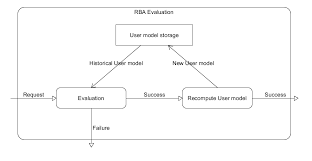
\includegraphics[width=0.8\textwidth]{BAB_TESIS/IMAGES/rba.png}
    \caption{Skema M2M Authentication}
    \label{fig:rba}
\end{figure}